\documentclass[11pt]{extarticle}
\usepackage{fullpage}
\usepackage[ampersand]{easylist}
\ListProperties(Hide=10, Style*=$\bullet\;\,$, Style2*=$\;\,${\tiny$\blacksquare$}$\;\,$,Space*=1mm,Space2*=0.1mm)

\usepackage{hyperref}
\hypersetup{colorlinks=true,
	linkcolor=black,
	filecolor=black,      
	urlcolor=black}
	
\usepackage{amsmath,amssymb,amsthm,mathtools,mathrsfs}
\newtheorem{thm}{Theorem}[]
\usepackage{bibref}

\usepackage[T1]{fontenc}
\usepackage[sc,osf]{mathpazo}
\usepackage{eulervm}

\usepackage{tikz}
\usetikzlibrary{calc}
\usetikzlibrary{shapes}
\usepackage{pgfplots}
\pgfplotsset{trig format plots=rad}
\usetikzlibrary {3d}
\pgfplotsset{compat=1.18}

\usepackage{multicol}
\setlength{\columnsep}{5mm}
\setlength\columnseprule{.1pt}

\usepackage[most]{tcolorbox}
\tcbuselibrary{skins}
\usepackage[explicit]{titlesec}
\newtcolorbox{secbox}[1][]{enhanced,attach boxed title to top center,drop fuzzy shadow,breakable,colbacktitle=gray,colback=black,colframe=black,
	coltext=white,size=title,title={#1}}
\titleformat{\section}[runin]{\bfseries\LARGE}{}{0pt}{\hfill
	%\begin{secbox}[\thesection]
	%	\centering #1
	%\end{secbox}
	%}
\tcbsidebyside[sidebyside adapt=left,segmentation style=solid,enhanced,size=small]
{%
	\thesection 
}
{%
	#1
}
}
\titleformat{\subsection}[runin]{\bfseries\large}{}{0pt}
{\hfill
%	\begin{secbox}[\thesubsection]
	%		\centering #1
	%	\end{secbox}
\tcbsidebyside[sidebyside adapt=left,segmentation style=solid,enhanced,size=small]
{%
	\thesubsection 
}
{%
	#1
}
}
\titleformat{\subsubsection}[runin]{\bfseries}{}{0pt}
{\hfill
%		\begin{secbox}[\thesubsubsection]
	%			\centering #1
	%		\end{secbox}
\tcbsidebyside[sidebyside adapt=left,segmentation style=solid,enhanced,size=small]
{%
	\thesubsubsection 
}
{%
	#1
}
}

\newcommand{\R}{\mathbb{R}}
\newcommand{\C}{\mathbb{C}}
\newcommand{\Na}{\mathbb{N}}
\newcommand{\Z}{\mathbb{Z}}
\newcommand{\F}{\mathbb{F}}
\newcommand{\Q}{\mathbb{Q}}
\newcommand{\ra}{\rightarrow}
\newcommand{\w}[1]{\text{#1}}
\newcommand{\ck}{.\,.\,}
\newcommand{\sm}[2]{\displaystyle\sum_{#1}^{#2}}
\newcommand{\Uint}[2]{\overline{\int\!}_{#1}^{\;#2}}
\newcommand{\Lint}[2]{\underline{\int\!}_{\;#1}^{\;#2}}
\newcommand{\pfrac}[2]{\frac{\partial#1}{\partial#2}}
\newcommand{\ckfil}{$.\dotfill.$}
\newcommand{\snote}[1]{{\footnotesize(#1)}}
\newcommand{\st}{\,{}_{s}|_t\,}
\newcommand{\tm}{\times}
\newcommand{\smdp}{ \,

\begin{tikzpicture}
	\draw[thick] (0,0)--(1ex,1ex)--(1ex,0)--(0,1ex);
\end{tikzpicture} 
\,
}
\newcommand{\gen}[1]{\langle #1 \rangle}
\newcommand{\pst}{ \,\rotatebox[origin=c]{90}{$ \gen{||} $} \,}
\newcommand{\tbx}[2][]{
\begin{tcolorbox}[enhanced,breakable,size=small,colback=black!2!white,title={#1},arc is angular, arc=1.5mm,drop fuzzy shadow]
	#2
\end{tcolorbox}
}
\newcommand{\rai}{\xrightarrow{\sim}}
\newcommand{\y}{$\blacksquare\;$}

\author{Yashas.N}
\title{Field \& Galois Theory}
\date{}

\begin{document}
	\maketitle
	\boldmath
	\begin{multicols}{2}
	
	\section{Field Extension \\ Theory}
\tbx[\textbf{Prime Subfield}]{of a Field $ F $ is a subfield of $ F $ generated by its multiplicative identity $ 1 $. We know that this is isomorphic to $ Q $ or $ \Z/pZ(=\mathbb{ F }_p) $ depending on the Characteristic of 
		$ F $ ($ch(F)$).
		} 
\tbx{If $ K $ is a field containing a subfield $ F $ then $ K $ is said to be the extension field or extension of $ F $ Denoted by $ K/F $ \snote{not to be confused with quotient group.}
		} 
\tbx[\textbf{Degree or Index} ]{of a field extension $ K/F $ is the dimension of $ K $ as a Vector space over $ F $ and is denoted by $ [K:F] $ 
		} 
\tbx[\textbf{Existence of Extension} : ]{ if $F$ is a field and and $ p(x) \in F[x]$ be an irreducible polynomial then
		there exists a field $K $ containing an isomorphic copy of $F$ in which $p(x)$ has a root. \\
		\snote{Given by $ K=F[x]/(p(x)) $ where $ \pi : F[x]\ra F[x]/(p(x)) $ is considered and $ x\ra \theta $ then $ p(\theta)=0 $ in $  K $ .}
		} 
\tbx{if $ p(x)\in F[x] $ is irreducible polynomial of degree $ n $ over field $ F $, field $ K= F[x]/(p(x)) $ and $ \theta = x\pmod{p(x)} \in K$ then $ \{1,\theta,	\theta^2,\ck , \theta^{n-1}\} $ forms a basis of vector space $ K $ over $ F $ i.e. $ [K:F]=n $ and 
		\begin{center}
			$ K=\{a_0+a_1\theta+a_2\theta^2+\ck +a_{n-1}\theta^{n-1}| a_i \in F\} .$
		\end{center}  
		} 
\tbx[Operations in field extension via $ p(x) $]{
\y addition is usual polynomial addition\\
\y  multiplication is defined as $ a(\theta)b(\theta)=r(\theta) $ where $ a(x)b(x) $ is multiplied in $ F[x] $ and divided by $ p(x) $ to give remainder $ r(x) $ which gives $ r(\theta) $ \\
\y as $ K $ is field each element has an inverse to find $ a^{-1}(\theta) $ : as $ p(x) $ is irreducible in $ F[x] $ and degree $ a(x)< $ degree $ p(x) $ we have $ (a(x),p(x))=1 \implies \exists b(x),c(x)\in F \st b(x)a(x)+c(x)p(x)=1$, now $ \pmod{p(x)} $ this we get $ b(x)a(x) \equiv 1\pmod{p(x)}$ i.e. 
		$ a^{-1}(\theta)=b(\theta) .$}
		
\tbx[$ F(\alpha,\beta,\ck) $]{ if $ \alpha,\beta,\ck \in K $ for some field extension $ K $ of $ F $ then the smallest subfield of $ K $ containing $ F $ and $  \alpha,\beta,\ck $ is called \textbf{field generated} by $ \alpha,\beta,\ck  $ over $ F $ denoted by $ F(\alpha,\beta,\ck ) $ i.e. for eg $ F(\alpha) $ is nothing but the smallest field containing both $ F $ and $ \alpha $ with condition that it is known some extension of $ F $ contains $ \alpha $.
		} 
\tbx[Simple extension]{if $ K $ field extension of $ F $ is such that $ K=F(\alpha) $ 
		} 
\tbx{if $ K $ field extension of $ F $ is such that for $ p(x)\in F[x] $ irreducible and root $ \alpha $ of $ p(x) $ is contained in $ K $ i.e. $ p(\alpha)=0 $ in $ K $ then for $ F(\alpha) $ subfield generated by $ F,\alpha $ in $ K $ we have  
	\[F(\alpha)\cong F[x]/(p(x)) .\] in $ K $ }
\tbx{	so we get 
		\[  F(\alpha)=\{a_0+a_1\theta+a_2\theta^2+\ck \]\[+a_{n-1} \theta^{n-1}| a_i \in F \}.\]
		\snote{Note : according to this any roots of $ p(x) $ are indistinguishable algebraically i.e. if $ \alpha,\beta $ are roots same irreducible $ p(x) $ in $ F[x] $ then $ F(\alpha)\cong F(\beta) $.}
		} 
\tbx{if $ F\cong F' $ (both fields) by isomorphism $ \phi  $ denoted by $ \phi : F \rai F'$ , 
	$ p(x)\in F[x] $ irreducible, $ p'(x)=\phi(p(x))\in F'[x] $ 
		and for $ \alpha $ a root of $p(x) $ (in some extension), $ \beta $ a root of $ \phi(p(x))$ (in some extension) then there exist an isomorphism $ \sigma : F(\alpha)\ra F'(\beta) $ extending $ \phi $ (restriction of $ \sigma $ to $ F $ $ : \, \sigma|_K $ is $ \phi $) which maps $ \alpha  \ra \beta$. i.e.
		\begin{center}
			if $ \phi : F \rai F' $\\
			$\st \alpha$ root of $p(x)$ , $ \beta$ root of $\phi(p(x))$\\
			then $\exists \sigma : F(\alpha)\rai F'(\beta)$\\
			by $ \alpha \ra \beta $ and $ \sigma|_F=\phi $  
		\end{center} 
 represented as 
\begin{center} 
		$\begin{matrix}
 	\sigma : & F(\alpha)&\rai&F'(\beta)\\
 	&|&&|\\
 	\phi : & F & \rai & F'
 	\end{matrix}$ 
 \end{center}
}
 \subsection{Algebraic Extensions}
\tbx[Algebraic ]{an element $ \alpha \in K $ extension of $ F $ is said to  algebraic over $ F $ if $ \alpha $ is root of 
		some non zero $ f(x)\in F[x]  $}
\tbx[Transcendental ]{		if $ \alpha $ is non algebraic then it is said to be transcendental over $ F .$ 
		} 
\tbx[Algebraic extension]{The extension $ K/F $ is called algebraic if every element of $ K $ is algebraic over $ F .$
		} 
\tbx[Minimal polynomial]{ if $ \alpha $ is algebraic over $F$ then there is unique monic irreducible polynomial $ m_{\alpha,F}(x)\in F[x] $ called \textbf{minimal polynomial} for $ \alpha $ over $ F $, which has $ \alpha $ as a root and if $  f(x)\in F[x]$ has $ \alpha $ as a root then $ m_{\alpha,F}(x) $ divides $ f(x) $ in $ F[x] $.\\
		$ m_{\alpha,F} (x)$ is simply written as $ m_\alpha(x) $ if $ F $ is known and degree $ m_\alpha $ is called 
	\textbf{	degree of $ \alpha $ }
		} 
\tbx{if $ L/F $ is an extension of fields and $ \alpha $ is algebraic over both $ F,L $ then $ m_{\alpha,L}(x) $ divides $ m_{\alpha,F}(x) $ in $ L[x] $ \snote{as $ m_{\alpha,F}(x) $ is also a polynomial with root $\alpha$ in $ L[x] $.}
		} 
\tbx{If $ \alpha $ is algebraic over $ F $ then 
		\begin{center}
			$ F(\alpha)\cong F[x]/(m_{\alpha,F}(x)) $,\\
			$ [F(\alpha):F]= $ degree $ m_{\alpha,F}=  $ degree $ \alpha. $ 
		\end{center}  
	} 
\tbx{$\alpha$ is algebraic over $ F $ iff the simple extension $ F(\alpha)/F $ is finite i.e. of finite dimension.\\
	more precisely if $ \alpha  $ is an element of an extension of degree $ n $ over $ F $ then $ \alpha $ satisfies a polynomial of degree at most $ n $ over $ F $ conversely  $ \alpha $ satisfies a polynomial of degree $ n $ over $ F $ then the degree of $ F(\alpha) $ over $ F $ is atmost $ n $.
	} 
\tbx{if extension $ K/F $ is finite then it is algebraic.
	} 
\tbx{if $ F\subseteq K \subseteq L $ are fields then 
	\begin{center}
		$ [L:F]=[L:K][K:F] .$
	\end{center} in particular degree of $ K/F $ divides degree of $ L/F $ 
	\\ \snote{holds even if degrees are infinite}
	} 
\tbx{extension $ K/F $ is finitely generated if $ K=F(\alpha_1,\alpha_2,\ck , \alpha_k) .$ for some $ \alpha_1,\alpha_2,\ck , \alpha_k \in K .$\\
 $ F(\alpha,\beta) =(F(\alpha))(\beta)$ i.e. $ F(\alpha_1,\alpha_2,\ck , \alpha_k)  $ can be inductively defines as 
	$ F((\alpha_1,\alpha_2,\ck \alpha_{k-1}))(\alpha_k) .$
	} 
\tbx{extension $ K/F $ is Finite iff $ K $ is generated by finite number of algebraic elements over $ F $\\
	more precisely a field generated over $ F $ by finite number of algebraic elements of degree $ n_1,n_2,\ck ,n_k $ is algebraic of degree $ \leq n_1n_2\ck n_k .$
	} 
\tbx{if $ \alpha ,\beta $ are algebraic  over $ F $ then $ \alpha+\beta , \alpha\beta ,\alpha^{-1}=1/\alpha,\alpha/\beta $  belong to same $ F(\alpha,\beta) $(field), thus are algebraic.
	} 
\tbx{in extension $ L/F $ the collection of algebraic elements over $ F $ forms a subfield.
	} 
\tbx{if $ K $ is algebraic over $ F $ and $ L $ is algebraic over $ K $ then $ L $ is algebraic over $ F .$ 
	} 
\tbx[Composite field]{if $ K_1,K_2 $ are sub fields of $ K $ then let $ K_1K_2 $ denote the smallest subfield of $ K $ containing both $ K_1, K_2.$ 
	\\
if $ K_1,K_2 $ be two finite extensions of $ F $ contained in $ K $ then
\[ [K_1K_2:F]\leq  [K_1:F][K_2:F].\]
equality holds iff $ F- $ basis elements of one field is linearly independent of the other.\\

if $[K_1:F]=n,[K_2:F]=m$ and $ (n,m)=1 $ then $ [K_1K_2:F]=nm=  [K_1:F][K_2:F].$
    } 
\tbx[Quadratic Extension of fields with \\ characteristics $ \neq 2 $  ]{ 
    If $ [K:F]=2 $ an $ \alpha $ is any element of $ K $ not in $ F $ then 
    $ m_\alpha(x)= x^2+bx+c \w{ for } b,c \in F$ note degree $ m_\alpha(x) \neq 1$ as it 
    means $ \alpha \in F$. Now $ F\subseteq F(\alpha)\subseteq K $ and $ [F(\alpha):F]=2 $,Thus $ K=F(\alpha) .$\\
    Now $\alpha= -b\pm \sqrt{b^2-4c}/{  2}$  so as $ F $ is not of Characteristic 
    $2 $ we can divide by $ 2 $ so we get $ F(\alpha) = F(\sqrt{b^2-4c})  $ where 
    $ b^2-4c $ is not a square in $ F $. Thus \textbf{ all extension of Degree $ 2 $ of 
    $ F $ is of form $ F(\sqrt{D})$ }  for some non square $ D $ in $ F.$}
\tbx[Splitting Field]{The extension field $ K $ of $ F $ is a splitting field of $ f(x)\in F[x] $ if $ f(x) $ factors completely into linear factors in $ K[x] $ and $ f(x) $ does not factor completely  into linear factors over any proper subfield of $ K $ containing $ F .$ i.e. $ K $ is the minimal field extension of $ F $ containing all roots of $ f(x)\in F[x] $ }
\tbx[Existence of Splitting Field]{ every $ f(x)\in F[x] $ has a splitting field. \snote{use induction on degree of polynomial}}
\tbx{Splitting field of a polynomial of degree $ n $ over $ F $ is degree at most $ n! $ over $ F .$   }
\tbx{  if $ \phi : F \rai F' $ is isomorphism of fields, $ f(x)\in F[x] $ , $ \phi(f(x)) = f'(x) \in F'[x] $ , $ E $ is splitting field of $ f(x)\in F[x] $ and $ E' $ is splitting field of $ f'(x)\in F[x] $ then there exist isomorphism $ \sigma: E \rai E' $ that extends $ \phi .$ i.e.
\begin{center}
		$ \begin{matrix}
	\sigma : & E&\rai&E'\\
	&|&&|\\
	\phi : & F & \rai & F'
	\end{matrix} $
\end{center}
}
\tbx{ Any two splitting fields for a same polynomial $ f(x)\in F[x] $ over $ F $ are isomorphic  }
\tbx[Algebraic closure]{ Field $ \bar{F} $ is called the closure of $ F $ if $ \bar{F} $ is algebraic over $ F $ and every polynomial $ f(x)\in F[x] $ splits completely over $ F .$   i.e. $ \bar{F} $ contains all the algebraic elements of $ F .$ }
\tbx[Algebraically closed]{ Field $ K $ is algebraically closed if every polynomial with coefficients in $ K $ has a root in $ K .$   }
\tbx{if $ \bar{F} $ is algebraic closure of a field $ F $ then $ \bar{F} $ is algebraically closed. }
\tbx[Existence of Algebraic closure]{ Every field $ F $ contains a algebraically  closed field $ K $ containing $ F $ \\
\snote{use Artin's proof : for every monic poly $ f(x)\in  F[x]$ denote $ x_f $ as an indeterminate and in ring $ F[\ck,
x_f,\ck] $ (an infinite variable polynomial field) prove ideal $ I=\gen{\ck,f(x_f),\ck} \forall f$ is proper thus contained in some maximal ideal $ M $ , let $ K_1 =F[\ck , x_f,\ck ]/M$ (quotient) clearly $ K_1 $ contains an isomorphic copy of $ F $ and every poly $ f \in F[x]$ has a root  in $ K_1 $ namely $ x_f $ performing this same process to $ K_1 $ and further we get $ F=K_0\subseteq K_1 \subseteq K_2 \ck \subseteq K_j \subseteq K_{j+1} \subseteq\ck  $ (not direct subsets but isomorphic) and let $ K= \underset{j\geq 0}{K_j}$ the $ K $ is algebraically closed and contains $ F $ \\
Now if $ K $ is algebraically closed field containing $ F $ then $ \bar{F} \subseteq K$ containing elements of $ K $ algebraic over $ F$ is the algebraic closure of $ F.$  }}
\subsection{Separable and Inseparable\\ Extensions}
%\tbx{ if $ f(x)=(x-a_1)^{n_1}(x-a_2)^{n_2}\ck (x-a_k)^{n_k} \in F[x] $ for $ a_i's $ distinct elements in the splitting field $ a_i $ is called a multiple root if $ n_i>1 $ with multiplicity $ n_i $ of $ f(x) $ or is simple root of $ f(x) $  if $ n_i=1 $ }
\tbx[Separable and Inseparable]{ A polynomial $ f(x)\in F[x] $ is separable if it has no multiple roots i.e. all its roots are distinct and has no repeated roots, if $ f(x) $ is not separable then it is inseparable.}
\tbx[Algebraic definition of Derivative ]{ if $ f(x)=a_nx^n+a_{n-1}x^{n-1}+\ck +a_1x+a_0 \in  F[x]$ define\\
$ D_xf(x)= na_nx^{n-1}+(n-1)a_{n-1}x^{n-2}+\ck+2a_2x+a_1\in F[x]. $  \\
\snote{$ D_x $ is usual analytic derivative w.r.t $ x $ but it can also viewed as a linear function on $ F[x] $ by above definition so usual rules and properties \snote{like product rule of derivative } follow even if there is no notion of `limit' or any other analytical terms.}}
\tbx[Test for multiple root]{ $ f(x) $ has a multiple root $ \alpha $ iff $ \alpha $ is also a root $ D_xf(x) $ \\
i.e. if $ \alpha $ is the root of both $ f(x),D_xf(x) $ i.e. the minimal polynomial of $ \alpha $ divides both $ f(x),D_xf(x) $ then $ \alpha $ is multiple root of $ f(x) $}
\tbx{ Every irreducible polynomial over a field of characteristic $ 0$ is separable, A polynomial over such a field is separable iff it is a product of distinct irreducible polynomial \\
\snote{use $ D_x p(x) $ is of degree less than one of degree of $ p(x) $ a irreducible so must be relatively prime i.e. $ (p(x),D_xp(x))=1 $, and as distinct irreducible polynomials are relatively prime in char 0 field the second statement follows}
}
\tbx[Frobenius endomorphism]{  if $ F$ is field of characteristic $ p $ then $ \forall a,b\in F $ \\
$ (a+b)^p=a^p+b^p,\; (ab)^p=a^pb^p $ \\
so the map $ \varphi : F\ra F $ by $ \varphi(a)=a^p $ is injective homomorphism }
\tbx{ if $ F $ is a finite field with characteristic $ p $ then every element of $ F $ is a $ p^{th} $ power in $ F $ i.e. Frobenius endomorphism is bijective in $ F $ this is denoted by $ F=F^p $ \snote{as the map is not trivial} }
\tbx{ Every irreducible polynomial over a finite field $ F $ is separable  and a polynomial in $ F[x] $ is separable iff it is product of distinct irreducible polynomials in $ F[x] $ \\
\snote{the only problem that may occur is if $ D_xp(x)=0 $ in this case if $ Char\; F=p $ then $ p(x)=q(x^p) =a_m(x^p)^m+\ck +a_0=b_m^p(x^p)^m+\ck +b_0^p=(b_mx^m+\ck +b_0)^p$ by frobenius endomorphism thus a contradiction to $ p(x) $ being reducible }}
\tbx[Separable extension]{  $ K $ is said to be separable over  $ F $ if every element of $ K $ is a root of separable polynomial over $ F $  }
\tbx[Perfect Fields]{ A field $ K $ is perfect if it is of characteristic $ p $ and every element of $ K $ is $ p^{th} $ power in $ K .$ And any field of characteristic $ 0 $ is perfect.  }
\tbx{Every finite extension of a perfect field is separable. In particular, every finite extension of either $\Q$ or a finite field is separable. }
\subsection{Finite fields}
\tbx{$ Z_p =\Z/p\Z$ is a finite field of characteristic $ p $ for prime $ p $ and is minimal field of characteristic $ p $ i.e. any field $ \F $ with characteristic $ p $ contains an isomorphic field to $ Z_p $}
\tbx{if $ \F $ is a finite field then it is of characteristic $ p $ a prime in $ \Z^+ $}
\tbx{ if $ \F $ is finite field of characteristic $ p $ then $ |\F|=p^n $ for some $ n\in \Z^+ $ \\
\snote{use : $ \F $ is a finite vector field over $ Z_p $ as $ Z_p\subseteq \F $ (the subfield generated by $ 1\in \F $ ) thus finite dimensional so $ [\F:Z_p]=n <\infty$ } }

\tbx{ $ x^{p^m}-x $ is separable over $ Z_p[x] $ with exactly $ p^m$ roots (in some extension)\\
Now the roots of this polynomial is closed under addition, subtraction, multiplication, and inverses so is the splitting field of   $ x^{p^m}-x $ thus \\
Finite fields of any order $ p^n $ exists and is unique upto isomorphism. So is denoted by $ \F_{p^n} $ \snote{the notation leads to $ Z_p=\F_p $ }}
\tbx[Representation of Finite fields]{From all above points we get that 
\begin{align*}
		(\F_{p^n},+)& \cong \overbrace{Z_p\tm Z_p \tm \ck \tm Z_p}^{n\w{ times}}.\\
	(\F_{p^n}^*,\tm)&\cong Z_{p^n-1}.
\end{align*}  }
\tbx{
	\y $ A $ is a subfield of $ \F_{p^n} $ iff $ |A|=p^m $ for some divisor $ m $ of $ n $ \\
\y $ \F_{p^n}\cap \F_{p^m}=\F_{p^{(m,n)}} $   }

\subsection{Cyclotomic Extension }
\subsubsection{Preliminaries}
\tbx{$ d|n $ iff $ x^d-1 | x^n-1 $ \\
\snote{for converse use if $ n=qd+r $ then $ x^n-1=(x^{qd+r}-x^r)+(x^r-1) $}}
\tbx{ Roots of $ x^n-1 $ are of form $ e^{2\pi k i/n} $ for $ k=0,1,\ck,n-1 $  }
\tbx[$ n^{th} $ root of unity]{the splitting field of $ x^n-1 $ over $ \Q $  and as $ F^* $ is cyclic for any field $ F $ and the roots of unity in this field is closed under multiplication \snote{prove} so is generated by an element of $ \C .$ i.e. the roots of $ x^n-1 $ in $ Q $ form a cyclic group \snote{under multiplication}}
\tbx[Primitive $ n^{th} $ root of unity ]{  A generator of $ n^{th} $ root of unity is called primitive $ n^{th} $ root of unity\\
clearly there are precisely $ \varphi(n) $ (euler's $ \varphi $-function) primitive $ n^{th} $ root of unity (as the roots form a multiplicative cyclic group)}
%\tbx{ if  $ (m,n)=1 $ and $ \zeta_m,\zeta_n$ are primitive $ m^{th} $ and $ n^{th} $ root of unity then $ \zeta_m\zeta_n $ is the primitive $ mn^{th} $ root of unity.\\
%if $ d|n $ then $ \zeta_d^n=1 $ so $ \zeta_d\in \mu_d $ and $ \zeta_n^d $ is one the primitive $ (n/d)^{th} $ root of unity.    }
\subsubsection{Main Concept}
\tbx[Cyclotomic Field]{  if $ \zeta_n $ is primitive $ n^{th} $ root of unity then $ \Q(\zeta_n) $ is called cyclotomic field of $ n^{th} $ root of unity}
\tbx{ let $ \mu_n $ denote the group of $ n^{th} $ roots of unity over $ \Q $ (only the roots)\\
Define the $ n^{th} $ cyclotomic polynomial 
\begin{align*}
	 \Phi_n(x) & = \prod\limits_{\zeta \w{ primitive }\in \mu_n}(x-\zeta)\\
	& =\prod\limits_{\substack{1\leq a\leq n \\ (a,n)=1 }} (x-\zeta_n^a)
	\end{align*} }
	\tbx{
\footnotesize now 
\begin{align*}
	x^n-1 &= \prod\limits_{\zeta \in \mu_n} (x-\zeta)\\
	\w{if }d|n& \w{ then }\zeta_d^n=1 \w{ so}\\
	x^n-1 &= \prod\limits_{d|n}\;\prod\limits_{\substack{\zeta \in \mu_d \\ \zeta \w{ primitive} }} (x-\zeta)\\
	\implies x^n-1 &= \prod\limits_{d|n}\Phi_d(x).\\
	\implies n & =\sum\limits_{d|n} \varphi(d)
	\end{align*}
}
\tbx{ Cyclotomic Polynomial $ \Phi_n(x) $ is irreducible monic polynomial of $ \Z[x] $ of degree $ \varphi(x) $ \\
so the degree of Cyclotomic field of $ n^{th} $ root of unity over $ \Q $ is $ \varphi(n) $ i.e.
\[[\Q(\zeta_n):\Q]=\varphi(n)\] }

\section{Galois Theory}

\tbx{ An automorphism $ \sigma $  of $ K $ field is said to fix $ \alpha\in K $ if $ \sigma(
	\alpha)=\sigma\alpha=\alpha $ and $ \sigma $ fixes $ F $ if it fixes every element of $ F $ 
	\\ if $ K/F $ is a field extension let $ Aut(K/F) $ denote all the automorphisms of $ K $ that fix $ F. $ \\
	clearly $ Aut(K/F) $ is subgroup of $ Aut(K) $ 
	\snote{under composition as group operations.}}
\tbx[Permutation Property]{  if $ K/F $ is field extension and $ \alpha\in K $ is algebraic over $ F $ then for any 
$\sigma\in Aut(K/F)$, $ \sigma\alpha$ is a root of minimal polynomial for $ \alpha $ over $ F $ i.e.\\
$ Aut(K/F) $ permutes the roots of irreducible polynomials or any polynomial with coefficients in $ F $  having $ \alpha $ as a root also has $ \sigma\alpha $ as a root}
\tbx{ If $ H\ll Aut(K) $   \snote{$ H $ subgroup of $ Aut(K) $ } then the collection of elements $F$ that are fixed by all elements of $ H $ is a subfield of $ K. $ }
\tbx[Reversal property]{ 
\y if $ F_1\subseteq F_2 \subseteq K $ are subfields of $ K $ then $ Aut(K/F_2)\ll Aut(K/F_1) $  
and\\
\y if $ H_1\ll H_2\ll Aut(K) $ and associated fixed fields are $ F_1 $ of $ H_1 $, $ F_2 $ of $ H_2 $ then $ F_2\subseteq F_1 $ }

\tbx{ if $ E $ is the splitting field over  of $ f(x) \in F[x]$ then 
\[|Aut(E/F)|\leq [E:F]\] 
equality holds iff $ f(x) $ is separable over $ F $ 
\\
\snote{use induction on $ [E:F] $ }}
\tbx{ $ Aut(\R/\Q)=1 $ only\\
\snote{prove these elements are continuous thus are trivial} }
\tbx[Galois Extension]{ for $ K/F $ a finite extension then $ K $ is said to be Galois  over $ F $ and $ K/F $ is Galois extension if $ |Aut(K/F)|=[K:F] $ and the $ Aut(K/F) $ is called the Galois group of $ K/F .$ 
\snote{if $ K/F $ is Galois .}\\
clearly If $ K $ is splitting field over $ F $ of some separable polynomial in $ F[x] $ then $ K/F $ is Galois.}

\tbx{ If $ \sigma_1,\sigma_2,\ck , \sigma_n $ are distinct embeddings of a field $ K $ into a field $ L $ then These are linearly independent as functions on $ K $. }
\tbx{ if $ G=\{ \sigma_1=1,\sigma_2,\ck , \sigma_n \} $ is subgroup of $ Aut(K) $ for $ K $ field and if $ F $ is the fixed field of $ G $ then 
\[[K:F]=n=|G|\]  }
\tbx{ if $ K/F $ finite extension then  \[|Aut(K/F)|\leq [K:F]\]}
\tbx{from above two points we have if $ G $ is any finite subgroup of $ Aut(K) $, if $ F $ is the fixed field of $ G $ then $ K/F $ is  Galois with Galois group $ G. $ }
\tbx{ If $ G_1\neq G_2 $ are distinct finite subgroups of $ Aut(K) $ then their fixed fields are distinct }
\tbx[Alternative Definition of Galois Extension]{ 
$ K/G $ is Galois iff \\
\y  $ K $ is the splitting field of some separable polynomial over $ F. $ \\
(and Further more then ever irreducible polynomial with coefficients in $ F $ which has a root in $ K $ is separable and has all its roots in $ K $  )\\
\y $ F $ is precisely the set of elements fixed by $ Aut(K/F) $\\
 \snote{note: in general the fixed field maybe larger than $ F $ }}

\tbx[\textbf{Fundamental Theorem of Galois Theory }]{ if $ K/F $ is a Galois Extension and $ G=Gal(K/F)=Aut(K/F) $ then there is a bijection \\
	$\begin{Bmatrix}
	&	K\\
	\w{Subfields E}&	|\\
	\w{of }K &	E\\
	\w{containing }F&	|\\
	&	F\\
	\end{Bmatrix}
	\leftarrow\!\ra
	\begin{Bmatrix}
	&	\{1\}\\
	\w{\footnotesize Subgroups}&	|\\
	H \w{ of  }G &	H\\
	&	|\\
		& G\\
	\end{Bmatrix}$
	\\
	by  the correspondence\\
	$\begin{matrix}
		E& \ra &\begin{Bmatrix}
			\w{	\footnotesize The elements of }\\
			G \w{  fixing }E
		\end{Bmatrix}\\
		
		\begin{Bmatrix}
			\w{	The fixed field }\\
			\w{ of }H
		\end{Bmatrix} &
		\leftarrow & H 
	\end{matrix}$\\
With properties :\\
\y Inclusion reversal : if $ E_1,E_2 $ correspond to $ H_1,H_2 $ respectively then $ E_1\subseteq E_2 $ iff  $ H_2\ll H_1 $\\
\y $ [K:E]=|H| $ and $ [E:F]=|G:H| .$ \\
\y $ K/E $ is always Galois with $ Gal(K/E)=H .$ \\
\y $ E/F $ is Galois iff $ H $ is normal subgroup in $ G $ , then $ Gal(E/F)\cong G/H $(quotient group).\\
\y if $ E_1,E_2 $ correspond to $ H_1,H_2 $ respectively then $ E_1\cap E_2 $ corresponds to group $ \gen{H_1,H_2} $ and the composite field $ E_1E_1 $ corresponds to $ H_1\cap H_2 .$ \\
Diagrammatically \\
$ \begin{Bmatrix}
K &\leftarrow\!\!\!\ra& \{1\}&&\w{always Galois},\\
| && |& \ra & Gal(K/E)=H \\
E&\leftarrow\!\!\!\ra&H&&\\
|&& |&\ra &\w{Galios iff }\; H\trianglelefteq G, \\
F&\leftarrow\!\!\!\ra&G&&[E:F]=|G:H|\\
\end{Bmatrix}$ 
 }
\tbx[Galois Groups of finite field]{ 
 As any finite field is of form $ \F_{p^n} $ (unique upto isomorphism) for some prime $ p $ and integer $ n\geq 1 $ 
 and as this field is isomorphic to splitting field of $ x^{p^n}-x $ over $ \F_p $ so $ \F_{p^n}/\F $ is Galois with Cyclic Galois of order $ n $ ($ Z_n $)  which is generated by Frobenius automorphism $ \sigma_p  $ which maps $ a\mapsto a^p $ in $ \F_{p^n} $ i.e. 
 \[Gal(\F_{p^n}/\F_p) =\gen{\sigma_p}\]
 so which implies that finite field $ \F_{p^n} $ is a simple extension }
\tbx{  since even for finite field the splitting field of polynomial of type $ x^{p^n}-x $ has $ p^n $ elements, this can increase with $ n $ we get any \\
	\textbf{Any algebraically closed field must be infinite }}
\tbx{ if $ K/F $ is Galois extension and $ F'/F $ is any extension then $ KF'/F' $ is Galois extension with galois group\[Gal(KF'/F')\cong Gal(K/K\cap F')\] 
Diagrammatically \begin{center}
	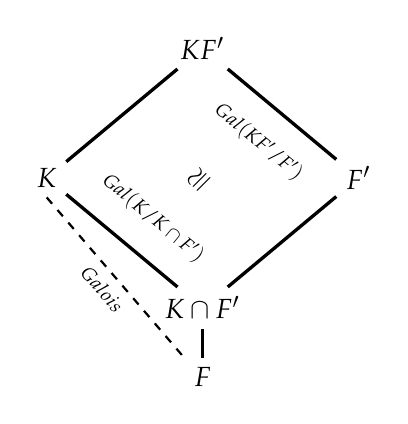
\begin{tikzpicture}[scale=1.1]
	\node (AB) at (0,1.5){$KF'$};
	\node (A) at (-1.8,0){$K$};
	\node (B) at (1.8,0){$F'$};
	\node (ab) at (0,-1.5){$K\cap F'$};
	\node (e) at (0,-2.3){$ F$ };
%	\node [scale=.7](NA) at (-1.5,1.9){{\boldmath$ N_G(B) $ }};
	\node at (0,0) {\rotatebox[origin=c]{45}{$ \cong $  }};
	\draw 	(AB) edge[-,very thick] (A)
%	(NA) edge[-,very thin](A)
%	(NA) edge[-,very thin](G)
	(AB) edge[-,very thick] node [below, scale=1, sloped, yshift=-2mm] {\scriptsize$Gal(KF'/F')$} (B)
	(ab) edge[-,very thick] node [above , scale=1, sloped, yshift= 2mm] {\scriptsize$\quad Gal(K/K\cap F')$} (A)
	(ab) edge[-,very thick] (B)
	(ab) edge[-,very thick] (e)
	(A.south) edge[-, dashed , thick] node[below,sloped] {\scriptsize$Galois$}  (e.north west);
\end{tikzpicture}
\end{center}
 }
\tbx{ if $ K/F $ is Galois extension and $ F'/F $ is any extension then 
\[[KF':F]=\frac{   [K:F][F':F] }{[K\cap F':F]}\] }

\tbx{ if $ K_1/F $ and $ K_2 /F$ are Galois extensions then \\
$ K_1\cap K_2 $ is Galois over $ F $ \\
$ K_1K_2 $ composite field is Galois over $ F $ and is isomorphic to subgroup \\
$ H=\{(\sigma,\tau)| \sigma|_{K_1\cap K_2}=\tau|_{K_1\cap K_2}$ for $\sigma\in Gal(K_1/F),
\, \tau\in Gal(K_2/F)\}$   \\
Diagrammatically \begin{center}
	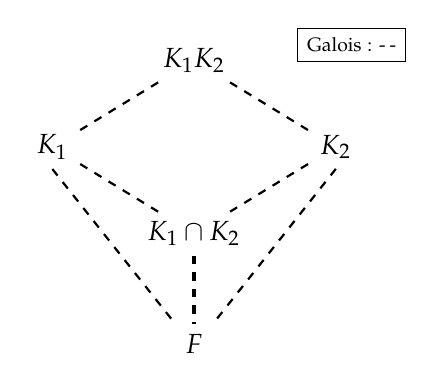
\begin{tikzpicture}[scale=1]
		\node[draw] at (2,1.3) {\scriptsize Galois : -\hspace{.5mm}- };
%		\node[draw] at (1.9,1.6) {\scriptsize};
		\node (AB) at (0,1.1){$K_1K_2$};
		\node (A) at (-1.8,0){$K_1$};
		\node (B) at (1.8,0){$K_2$};
		\node (ab) at (0,-1.1){$K_1\cap K_2$};
		\node (e) at (0,-2.5){$ F$ };
		%	\node [scale=.7](NA) at (-1.5,1.9){{\boldmath$ N_G(B) $ }};
		\draw 	(AB) edge[-,dashed,thick] (A)
		%	(NA) edge[-,very thin](A)
		%	(NA) edge[-,very thin](G)
		(AB) edge[-,dashed,thick](B)
		(ab) edge[-,dashed,thick] (A)
		(ab) edge[-,dashed,thick] (B)
		(ab) edge[-,dashed,very thick] (e)
		(A.south) edge[-, dashed , thick] (e.north west)
		(B.south) edge[-, dashed , thick]   (e.north east);
	\end{tikzpicture}
\end{center}
and if $ K_1\cap K_2=F $ we have\[Gal(K_1K_2/F)=Gal(K_1/F)\times Gal(K_2/F)\]}
\tbx[Galois Closure]{ if $ E/F $ is any finite extension then there exist a Galois extension $ K $  of $ F $ containing $ E $ and is minimal extension i.e. if there is any other such extension $ K_1 $ then $ K_1 $ contains an isomorphic subfield to $ K $ which again is Galois over $ F $ , here $ K $ is called Galois closure of $ E $ over $ F $ \\
\snote{use : the composite of splitting fields of minimal polynomial of basis elements of $ E $ over $ F $ is such extension. }  }
\tbx[Defining property of Simple extension ]{  if $ K/F $ is finite extension  then is simple extension i.e. $ K=F(\alpha) $ iff there are only finitely many subfields of $ K $ containing $ F .$ }
\tbx[Primitive element Theory]{ if $ K/F $ is finite and separable then $ K/F $ is simple extension.\\
In particular any finite extension of fields of characteristics $0$ (or any perfect field)  is simple extension\\
\snote{use : $ K $ is the finite subgroup of  Galois closure of $ K $ over $ F $ so as there are only finitely many subgroups of this group in the galois group and above point.} }
\tbx[Cyclotomic Extensions theory]{ Clearly $ \Q(\zeta_n)/\Q $ is Galois \snote{ for $ \zeta_n $ a primitive $ n^{th} $ root of unity}\\
   and $ Gal(\Q(\zeta_n)/\Q)\cong (\Z/n\Z)^* $ this isomorphism is given by
   $ \sigma \ra a\pmod{n} $ where $ \sigma_a\in Gal(\Q(\zeta_n)/\Q) $ is defined as $ \sigma_a(\zeta_n)=\zeta_n^a $ \\
   \snote{this is the case as all elements of galois group map the primitive element to another primitive element thus $ (n,a)=1 $ only.}}
  \tbx{  if $ n=p_1^{a_1}p_2^{a_2}\ck p_k^{a_k} \; \in \Z $ where $ p_i's$ are prime in $ \Z, a_i\in 
  	\Z^+ $ then 
  	\begin{center}
  		$  Gal(\Q(\zeta_n)/\Q)\cong Gal( \Q(\zeta_{p_1^{a_1}} )/\Q) \tm Gal( \Q(\zeta_{p_2^{a_2}} )/\Q)  \tm \ck \tm Gal( \Q(\zeta_{p_k^{a_k}} )/\Q) . $
  \end{center} 
\snote{which in terms of isomorphism of rings (fields) is purely Chinese remainder theorem}}
\tbx[Abelian Extension]{ $ K/F $ is abelian extension if $ K/F $ is galois and $ Gal(K/F) $ the galois group is abelian.\\
By Fundamental Theorem of Finite abelian groups, Fundamental theorem of Galois theory and the existence of groups which contain cyclotomic product groups stated  above \snote{by C.R.T and number theory} we have
\\
if $ G $ is any finite abelian group then there is a subfield $ K $ of a Cyclotomic extension field with  
\[Gal(K/\Q)\cong G\]\\
And if $ K $ is some finite abelian extension of $ Q $ then $ K $ is contained in some Cyclotomic extension of $ \Q $ }
\tbx[Class field Theory]{ it is the study abelian extension of arbitrary finite extension $ F $ of $ \Q $ . The study of the arithmetic of such abelian extensions and
	the search for similar results for non-abelian extensions are rich and fascinating areas
	of current mathematical research.}

\subsection{Galois groups of polynomials}
\tbx{ To study polynoinals of finite degree with arbitrary coefficients from a field $ F $ we see the coefficients as indeterminates ( sort of like variables )  this type of study leads to several generalisations and ultimately classifying galios group of polynomials of small degree as can be seen below}
\tbx[elementary symmetric functions]{ if $ x_1,x_2,\ck ,x_n $ are indeterminates then  elementary symmetric functions $ s_1,s_2,\ck , s_n$ are defined by 
\begin{align*}
	s_1 &= x_1+x_2+\ck+x_k\\
	s_2 &= x_1x_2+x_1x_3+\ck+x_2x_3+x_2x_4+\\
	& \quad\ck+x_{n-1}x_n\\
	\vdots\\
	s_n&= x_1x_2\ck x_k\\
	\end{align*} }
\tbx{ Now general polynomial of degree $ n $ is polynomial whose roots $ x_1,x_2,\ck ,x_n $ are indeterminates i.e.\\
$ =(x-x_1)(x-x_2)\ck (x-x_n)\\
= x^n-s_1x^{n-1}+s_2x^{n-1}+\ck+(-1)^ns_n$ \\
which gives a relation of roots and elementary symmetric functions in these roots which also continues as follows}
\tbx{ $ F(x_1,x_2,\ck,x_n) $  is the splitting field of $ F(s_1,s_2,\ck,s_n) $ and clearly is Galois extension.}
\tbx{ now the symmetric group $ S_n $ acts on $ F(x_1,x_2,\ck,x_n) $ of all rational functions in n variables  by permuting the corresponding variables so by this we have \\
the fixed field of $ S_n $  acting on $ F(x_1,x_2,\ck,x_n) $ of all rational functions in n variables  is the field of rational functions in their elementary symmetric functions  $ F(s_1,s_2,\ck,s_n) $ 
\\
A rational function  $ f(x_1,x_2,\ck,x_n) $  is symmetric if is is not changed by any permutation in variables  $x_1,x_2,\ck,x_n$\\
\textbf{Any Symmetric function can be decomposed as rational function in elementary symmetric functions} }
\tbx[Existence of $ S_n $ Galois group]{ general polynomial of degree $ n $ $x^n-s_1x^{n-1}+s_2x^{n-1}+\ck+(-1)^ns_n$
over $ F(s_1,s_2,\ck,s_n) $ is separable with Galois group $ S_n $\\
 \snote{i.e. if there is no relations among $s_1,s_2,\ck,s_n $ the coefficients of a polynomial of degree $ n $ then the Galois group of the the field generated by its coefficients is $ S_n $ (the maximum of its kind)}}
\tbx[Discriminant]{ discriminant $ D $ of $ x_1,x_2,\ck x_n $ is \[D=\prod\limits_{i<j}(x_i-x_j)^2\]
 now clearly $ D $ is a symmetric function\\
 but $ \sqrt{D} $ is not and an element of $ S_n $ fixes $ \sqrt{D} $ iff it can be decomposed into even number of transpositions i.e. iff it is an element of $ A_n $ alternating group of $ S_n $  }
 \tbx{ Immediately from above point we get \\
 Galois group of $ f(x)\in F[x] $ is a subgroup of $A_n $ iff the discriminant $ D $ is a square of an element of $ F. $ \\
 \snote{ this is the case as $ \sqrt{D} $ is fixed by every element of galios group means that i.e. $ \sqrt{D}\in F $ }  \\ \snote{if $ D=0 $ for $ f(x) $ then there is a multiple root in $ f(x) .$}}
 
 \subsubsection{Galois groups Polynomials of degree small degree}
 \tbx[Polynomials of degree $ 2 $ ]{ let general polynomial of degree $ 2 $ be \\
 $f_2(x)= x^2+ax+b \in F[x]$ and if $ \alpha,\beta $ are its roots then \\
 discriminant $ D=(\alpha-\beta)^2=\alpha^2+\beta^2-2\alpha\beta=(\alpha+\beta)^2-4\alpha\beta=s_1^2 -4s_2= a^2-4b$ \\
 \y so if $ D=a^2-4b=0 $ then $ p_2(x) $ has multiple root\\
 i.e. $ f_2(x) $ is separable iff $ a^2-4b\neq 0 $ thus the Galois group is trivial \snote{$\{1\}$}
 \y now if $ 0\neq \sqrt{D}=\sqrt{a^2-4b}\in F $ i.e. $ D $ is a square in $ F $ then Galios group is a subgroup of $\{1\}=A_2\ll S_2=\Z/2\Z   $ again a  trivial group
 \y the only remaining case is when $ f_2(x) $ is irreducible in $ F[x] $ i.e. $ \sqrt{D}=
 \sqrt{a^2-4b} \notin F$ then the Galois group is whole $ S_2=\Z/2\Z $ with the splitting field $ F(\sqrt{D}) $ \\
 \snote{This theory is same as discussed in Quadratic extensions but in more general with out knowing the exact formula of the root}}

\tbx[Polynomials of degree $ 3$ ]{  let $ f_3=x^3+ax^2+bx+c $\\
substituting $ x=y- a/{3}  $ $ f_3(x) $ becomes $ g_3(y) =y^3+py+q$ for $ p=\frac{1}{3}(3b-a^2) $ $q=\frac{ 1 }{27} (2a^3-9ab+27c)$\\
for discriminant $ D $ :\\
let $u,v,w$ be the roots of $ g_3(y) $ then \\
$ g_3(y)=(y-u)(y-v)(y-w)=y^3+py+q $ so we have \\
$ D_yg(u)=(u-v)(u-w) \\
D_yg(v)=-(u-v)(v-w)\\
D_yg(w)=(u-w)(v-w)$ \\
now $ D=[(u-v)(u-w)(v-w)]^2 $ we have\\
$ D=-D_yg(v)\,D_yg(v),D_yg(w) $ and as $ D_yg(y) =3y^2+p$ we have\\
$ -D=(3u^2+p)(3v^2+p)(3w^2+p) \\
= 27(uvw)^2+9p(u^2v^2+u^2w^2+v^2w^2)+3p^2(u^2+v^2+w^2)\\
= 27(uvw)^2
+9p[(uv+uw+vw)^2-2uvw(u+v+w)]
+3p^2[(u+v+w)^2-2(uv+uw+vw)] $\\
$ \implies D= 27s_3^2+9p(s_2^2-2s_3s_1)+3p^2(s_1^2-2s_2) $ \\
now $ g_3(y)= y^3+py+q \implies s_1=0,s_2=p,s_3=-q$ \\
so $ D= -4p^3-27q^2\\ =a^2b^2-4a^3c-4b^3+18abc-27c^2$ by all substitutions.\\
\y if $ f_3(x) $ is reducible then it splits in $ F $ 
\y if it splits into $ 3 $ factors then obviously all roots lie in $ F $ and Galois group is trivial
\y if it splits into one linear and an irreducible quadratic then Galois group is order $ 2 $ i.e. $ \Z/2/Z $ 
\y now if whole  $ f_3(x) $ is irreducible in $ F $ then the degree of extension is atleast $ 3 $ so is a subgroup of order $\geq 3 $ in $ S_3 $ only possible cases are either $ \Z/3\Z=A_3 $ or $ S_3 $ 
\y now if $ D $ is a square i.e. $ \sqrt{D}\in F $ then Galois group is $ \Z/3\Z=A_3 $ which is cyclic thus the splitting field  of  $ f_3(x) $ is obtained by adjoining any one roots to $ F $ i.e. $ F(\theta). $
\y if $ \sqrt{D}\notin F $ then clearly the only remaining possibility is $ S_2 $ thus the Galois group is $ S_3 $ and the splitting firld of $ f_3(x) $ is of degree $ 6 $ over $ F $ thus is $ F(\theta,\sqrt{D}) $ for any one root $ \theta $ of $ f_3(x) $ and $ D $ discriminant. }
\tbx[Polynomial of degree $ 4 $ ]{let $ f_4(x)=x^4+ax^3+bx^2+cx+d $ \\
substituting $ x=y-a/4 $ $ f_4(x) $ becomes $ g_4(y) y^4+py^2+qy+r$ where $ p=\frac{ 1 }{8} (-3a^2+8b),\; q=\frac{ 1 }{8} (a^3-4ab+8c),\; r=\frac{ 1 }{256} (-3a^4+16a^2b-64ac+256d) .$ \\
for discriminant $ D $ :\\
if $ u_1,u_2,u_3,u_4$ are roots of  $g_4(y)$ then let\\
$ \theta_1=(u_1+u_2)(u_3+u_4)\\
\theta_2 =(u_1+u_3)(u_2+u_4) \\
\theta_3=(u_1+u_4)(u_2+u_3)$ \\
then any element of $ S_4 $ permutes $ \theta _i's$ only so the elementary symmetric functions in $ \theta_i's $ remain fixed by elements of $ s_4 $ thus these elementary functions are (if $ s_i $  denote that of $ g_3 $)}
\tbx{
$ s'_1=\theta_1+\theta_2+\theta_3=2(u_1u_2+u_1u_3+u_1u_4+u_2u_3+u_2u_4+u_3u_4) =2(s_2)=2p$ \\
$ s'_2= \theta_1\theta_2+\theta_2\theta_3+\theta_1\theta_3=p^2-4r$\\
$ s'_3=\theta_1\theta_2\theta_3=-q^2 $ 
so $ \theta_1,\theta_2,\theta_3$  are roots of \textbf{resolvent cubic }$h_3(x)=  x^3-2p+(p^2-4q) x^2+q^2$ }
\tbx{
observing $ \theta_1-\theta_2=u_1u_3+u_2u_4-u_1u_2-u_3u_4=-(u_1-u_4)(u_2-u_3) $ \\
 $ \theta_1-\theta_3=-(u_1-u_3)(u_2-u_4) $\\
 $ \theta_2-\theta_3=-(u_1-u_2)(u_3-u_4) $\\
 we have discriminant of $ g_4(x) $ is same as $ h_3(x) $ so\\
 $ D$ can be calculated by transform $ x=y-a/3 $ obtain $ p,q,r $ form resolvent cubic $ x^3-2p+(p^2-4q) x^2+q^2$ and finding its discriminant.}
 \tbx{
 \y Now if $ f_4(x) $ is reducible into 4  linear factors in $ F $ then Galois group is trivial.\\
 \y If $ f_4(x) $ factors into 1 linear and irreducible cubic then the cases reduces to that on cubic discussed above.
 \\
 \y If $ f_4(x) $ factors into 2 irreducible quadratic then the splitting field $ F(\sqrt{D_1},\sqrt{D_2})$ for $ D_1,D_2 $ discriminants of the irreducible factors and if $ D_1,D_2 $ do not differ by square factor i.e. $ \sqrt{D_1}\neq k \sqrt{D_2}$ for some $ k\in F $ then Galois group is isomorphic to $ \Z/2\Z\tm \Z/2 \Z $ i.e. Klein's 4-group $ V $ in which every element is of order $ 2 .$ \\
\y  If $ f_4(x) $ is irreducible then the degree of splitting field is atleast $ 4 $ so is Galois group $ G $ is a subgroup of $ S_4 $ whose order is divisible by $ 4 $ and $ G $ is transitive on roots i.e. applying automorphisms in galois groups to any given root we can get all other roots so the only possibilities are \\
$ S_4,A_4,\\
D_8=\{1, (1324), (12) (34) , (1423), (13)(24) \\
, (14) (23), (12), (34) \} $ (isomorphic Dihedral and Sylow-$ 2 $ subgroup and its 3 conjugate subgroups in  $ S_4 $ )\\
$ V=\{1,( 1 2) (34) , (13) (24) , (14) (23)\} $ (only subgroup isomorphic to Klein's 4-group in $ S_4 $  )
$ C=\{ 1 , ( 1234), ( 13)(24), (1432)\} $ (a cyclic group with its 3 other conjugate subgroups in $ S_4 $ )\\
now the splitting field of the resolvent cubic is a subfield of the quartic so Galois group $ G' $ of the resolvent cubic is a quotient group of $ G $ so we examine the action of subgroups on quotient to reduce possibilities as follows \\
(note $ V $ fixes all $ \theta_1,\theta_2,\theta_3  $ and $  D_8 $ fixes $ \theta_1 $ and its conjugate fix other roots of $ h_3 $ .)\\
 \y if resolvent cubic is irreducible and $ D $ is not a square in $ F $ so the $ G $ is not contained in $ A_4 $ and as $ G'=S_3 $ $ 6||G|$  the only possibility is $ G=S_4. $ \\
 \y if resolvent cubic is irreducible and $ D $ is not a square in $ F $ then $ G\ll A_4 $ and $ G'=A_3 $ so $ 3||G| $ the only possibility is $ G=A_4. $ \\
 \y now if resolvent cubic $ h_3 $ is reducible , and if $ h_3 $ has all roots in $ F $ then each element of $ G $ fixes 
 $ \theta_1\theta_2\theta_3 $ so the only possibility is $ G=V $ \\
 \y if resolvent cubic $ h_3 $ is reducible , and if  $ h_3(x) $ splits into linear and quadratic the any one root say $ \theta_1 $ is in $ F $ so is fixed by all elements of $ G $ and not other roots so $ G\not\subseteq V $ so $ G=D_8 $ or $ C $ one way to distinguish is observe that $ F(\sqrt{D}) $ is fixed field of elements of $ G $ in $ A_4 $ so \\
 $ D_8\cap A_4=V $ and $ C\cap A_4=\{1,(13)(24)\} $  and the first group $ V $ is transitive on roots of $ f_4 $ but the other is not thus $ f_4 $ is reducible over $ F(\sqrt{D}) $ iff $ G=D_8 $ and if not we get $ G=C $ thus we may determine this by factoring $ f_4(x) $ in $ F(\sqrt{D}) .$}
 
 
   \subsection{Solvable and Radical extension}
   
\tbx[Cyclic extension ]{ $ K/F $ field extension is cyclic if it is Galois and its Galois group  is cyclic.}
\tbx[Simple Radical Extensions]{  Extensions of a field $ F $ obtained by adjoining the $ n^{th} $ root of an element in $ F $ i.e. of type $ F(\sqrt[n]{a}) $ for $ a\in F .$}
\tbx{Since all the roots of the polynomial $x^n -a$	for $a \in F $ differ by factors of the $ n^{th}$ roots of unity, adjoining one such root will give a Galois extension if and only if this field contains the $n^{th}$ roots of unity. }
\tbx{ If $F $ field is of characteristic not dividing $n $ which contains the $n^{th} $ roots of unity. Then the extension $ F ( \sqrt[n]{a} ) $for $a \in F $ is cyclic over $F $ of degree	dividing $n$ .\\
\snote{prove the homomorphism $ \phi: Gal(F(\sqrt[n]{a})/F) \ra \mu_n $ $ n^{th} $ roots of unity group by $ \sigma\sqrt[n]{a}=\zeta_\sigma\sqrt[n]{a}\w{ for } \sigma \ra \zeta_\sigma$ is injective  }}
\tbx[Lagrange Resolvent]{ if  $ K/F $ is cyclic extension of degree $ n $ , $ F $ is not of characteristic dividing $ n $ i.e. $ ch(F)\not|n $ , $\sigma$ the generator of $ Gal(K/F) $, $\alpha \in K$ and for any $ n^{th} $ root of unity $ \zeta $ Lagrange resolvent is given by  \begin{center}
		$(\alpha,\zeta)=\alpha+\zeta\sigma(\alpha)+\zeta^2\sigma^2(\alpha)$\\
		$\qquad+\ck+\zeta^{n-1}\sigma^{n-1}(\alpha)$
	\end{center} 
now $ \sigma(\alpha,\zeta)=\zeta^{-1}(\alpha,\zeta) $ so $ \sigma(\alpha,\zeta)^n=(\alpha,\zeta) $ }   
\tbx{  Any cyclic extension of degree $ n $ over $ F $ of $ ch(F)\not|n $ which contains $ n^{th } $ root of unity is of form $ F(\sqrt[n]{a}) $ for some $ a	\in F .$  }
\tbx[Root Extension]{ for field $ F $ of characteristic $ 0 $ an element $ \alpha $ is algebraic over $ F $ and it can be solved in terms of radicals (addition, subtraction, multiplication and division ) if $ \alpha\in K $ which can be obtained by successive simple radical extensions like\\
$ F=K_0\subset K_2\subset \ck \subset K_s=K $ where $ K_{i+1} =K_i(\sqrt[n_i]{a_i})$ for some $ a_i\in K_i $ for $ i=0,1,2\ck ,s-1 $ such a Field $ K $ is called Root extension of $ F $ }
\tbx[Solvable by radicals]{a polynomial $ f(x)\in F[x] $ is solvable by radicals if all of its roots are solvable by radicals}
\tbx[Cyclicity and Root extension theorem]{ if $ \alpha $ is contained in root extension $ K $ of $ F $ then $ \alpha $ is contained in root extension which is Gaois over $ F $ and in resulting chain $ K_{i+1}/K_{i} $ is cyclic}
\tbx[Solvablity theorem ]{  Polynomial $ f(x) $ can be solved by radicals iff its Galois Group is a \textbf{Solvable Group} \\
\snote{refer group theory recall finite group is solvable iff there exist a chain in which each successive quotient group is cyclic as in above point }}
\tbx[Insovablity of quintic and higher degree polynomial]{ Clearly as $ S_n $ for $ n\geq 5 $ is not a solvable group and the existence of general polynomial with Galois group $ S_n $ proves the fact that polynomials of degree $ \geq 5 $ cannot be solved by radicals.\\
\snote{use $ A_n $ for $ n\geq 5 $ is non abelian simple group and show $ [S_n,S_n]=A_n $ and $ [A_n,A_n] =A_n$ thus the groups in derived series of $ S_n $ is never $ \{1\} $ so is $ S_n $ is not solvable (refer Derived series in Group theory)} }

\begin{thebibliography}{9}
 	\bibitem{DF}
 	David S. Dummit, Richard M. Foote : Abstract Algebra, John Wailey \& sons, 3, (2004).
\end{thebibliography}
	
	\end{multicols}
	
\end{document}
